\chapter{Teoria}
\label{ch:teoria}
Tässä osiossa lukijaa perehdytetään työn kannalta tärkeään teoriaan. Teoriaosuuden kokonaan lukemalla lukija ymmärtää, mitä IEC 61850 -standardi tarkoittaa sähköasemien kannalta ja mitä kaikkea se määrittää. Kuinka standardi määrittää viestien tilauksen, ja mitä malleja ja palveluita niihin liittyy. Työn lopullisessa toteutuksessa viestit prosessoitiin ja julkaistiin jonopalvelimelle myöhempää käyttöä varten. Teorian lopussa lukija perehdytetään jonopalvelimen toteukseen liityvään teoriaan. Teoriaosuus lukemalla lukija varmistaa että, ymmärtää ohjelmiston suunnittelu- ja toteutusvaiheessa käsitellyt käsitteet ja aiheet.


\section{IEC 61850 -standardi yhteiseen kommunikointiin}
Sähköasemilla nykypäivänä käytössä olevilla älykkäillä elektronisilla laitteilla (engl. Intelligent Electronic Device, lyhennetään IED) toteutetaan aseman toiminnalisuuden funktioita. Aseman toiminnallisuuteen liittyy sen kontrollointi ja suojaus. Aseman komponenttien suojauksen lisäksi, siihen kuuluu myös asemalta lähtevät sähkölinjat. Hyvä esimerkki sähköaseman suojauksesta on korkeajännitelinjan katkaisija, joka katkaisee virran linjasta vikatilanteissa, kuten linjan poikkimeno kaatuneen puun tai pylvään takia. Fyysistä katkaisijaa ohjaa aseman automatiikka, joka toteutetaan IED-laitteilla. Eli IED-laite voi olla kytketty fyysisesti ohjattavaan laitteeseen \cite[s.~63--64]{IEC61850-7-1}. Koko sähköaseman toiminnallisuus koostuu monesta funktiosta, jotka on jaettu monelle IED-laitteelle. Jotta systeemi pystyy toimimaan, täytyy IED-laitteiden kommunikoida keskenään ja vaihtaa informaatiota toistensa kanssa. IED-laitteiden täytyy myös kommunikoida asemalta ulospäin erilliselle ohjausasemalle monitorointia ja etäohjausta varten \cite[s.~1]{Brunner2008}. On selvää, että monimutkaisen systeemin ja monen valmistajien kesken tarvitaan yhteiset säännöt yhteistä kommunikointia varten.

Maailmanlaajuisesti määritetty IEC 61850 -standardi määrittää sähköaseman sisäisen kommunikoinnin IED-laitteiden välillä. Standardi määrittää myös kommunikointisäännöt asemalta lähtevään liikenteeseen, kuten toiselle sähköasemalle ja ohjausasemalle \cite[s.~10]{IEC61850-7-1}. Ilman yhteisiä sääntöjä jokainen valmistaja olisi vapaa toteuttamaan omat säännöt ja protokollat kommunikointiin. Seurauksena tästä olisi, että laitteet eivät olisi keskenään yhteensopivia eri valmistajien välillä. Standardin on tarkoitus poistaa tämä ja määrittää yhteiset pelisäännöt kommunikoinnin toteuttamiseen \cite[s.~1]{Kaneda2008}.

Todella tärkeä ja iso osa standardia on sähköaseman systeemin funktioiden abstrahointi mallien kautta. Standardi määrittää tarkasti kuinka abstraktit mallit määritellään aseman oikeista laiteista ja niiden ominaisuuksista. Tarkoituksena on tehdä mallit tekniikasta ja toteutuksesta riippumattomaksi. Tämän jälkeen abstrahoidut mallit mallinnetaan erikseen jollekin tekniikalle, joka sen mahdollistaa. Abtrahoituja malleja käytetään myös määrittämään sähköaseman IED-laitteiden ja aseman muiden osien konfigurointi. Abstrahoitujen mallien ansiosta standardi on pohjana tulevaisuuden laajennoksille ja tekniikoille. Uusien tekniikoiden ilmaantuessa, voidaan standardin lisätä  osa, joka  mallintaa abstraktimallit kyseiselle tekniikalle \cite[s.~2]{Brunner2008}. Teoriassa ensin käsitellään standardin asioita abstraktilla tasolla, liittämättä sitä mihinkään tekniseen toteutukseen. Vasta tämän jälkeen se liitetään erikseen tekniikkaan mitä työssä käytettiin.


\subsection{Standardin eri osat ja niiden merkitykset}	
IEC 61850 -standardi on todella laaja kokonaisuus. Tämän takia se on pilkottu erillisiin dokumentteihin, josta jokainen käsittelee omaa asiaa. Historian saatossa standardiin on lisätty uusia dokumentteja laajentamaan standardia \cite{IEC61850series, New-documents-by-IEC-TC-57} \cite[s.~13]{IEC61850-1}. Tämän työn kirjoitushetkellä standardiin kuului lisäki paljon muitakin dokumentteja, esimerkiksi uusiin mallinnuksiin muille tekniikoille ja vesivoimalaitoksien mallintamiseen liittyviä dokumentteja. Laajuudesta huolimatta standardin voi esittää 10:llä eri pääkohdalla ja näiden alakohdilla. Taulukossa \ref{tab:iec61850-dokumentin-osat} on esitetty standardin pääkohdan dokumentit ja niiden alkuperäiset englanninkieliset otsikot \cite[s.~2]{Mackiewicz2006} \cite{IEC61850series}. Kuvassa \ref{fig:iec61850-osat-ja-relaatiot} on esitetty kaikki standardin eri osat ja niiden väliset relaatiot toisiinsa. Kuvaan on merkitty yhteinäisellä viivalla ne osat, jotka ovat tämän työn kannalta tärkeitä. Ja katkoviivalla ne, jotka eivät ole.

\begin{table}[ht!]
	\caption{IEC 61850 -standardin pääkohtien ja niiden alakohtien dokumentit.}
	\label{tab:iec61850-dokumentin-osat}
	\begin{tabular}{l | l}
		\hline
		\textbf{Osa} & \textbf{Otsikko englanniksi} \\
		\hline \hline
		1 & Introduction and overview \\
		2 & Glossary \\
		3 & General requirements \\
		4 & System and project management \\
		5 & \parbox[t]{13cm}{Communication requirements for functions and device models} \\
		6 & \parbox[t]{13cm}{Configuration description language for communication in power utility \par automation systems related to IEDs} \\
		7-1 & \parbox[t]{13cm}{Basic communication structure - Principles and models} \\
		7-2 & \parbox[t]{13cm}{Basic information and communication structure - Abstract communication service interface (ACSI)} \\
		7-3 & \parbox[t]{13cm}{Basic communication structure - Common data classes} \\
		7-4 & \parbox[t]{13cm}{Basic communication structure - Compatible logical node classes and data object classes} \\
		8-1 & \parbox[t]{13cm}{Specific communication service mapping (SCSM) - \par  Mappings to MMS (ISO 9506-1 and ISO 9506-2) and to ISO/IEC 8802-3} \\
		9-2 & \parbox[t]{13cm}{Specific communication service mapping (SCSM) - \par  Sampled values over ISO/IEC 8802-3} \\
		9-3 & \parbox[t]{13cm}{Precision time protocol profile for power utility automation} \\
		10 & Conformance testing \\
		\hline
	\end{tabular}
\end{table}

\begin{figure}
	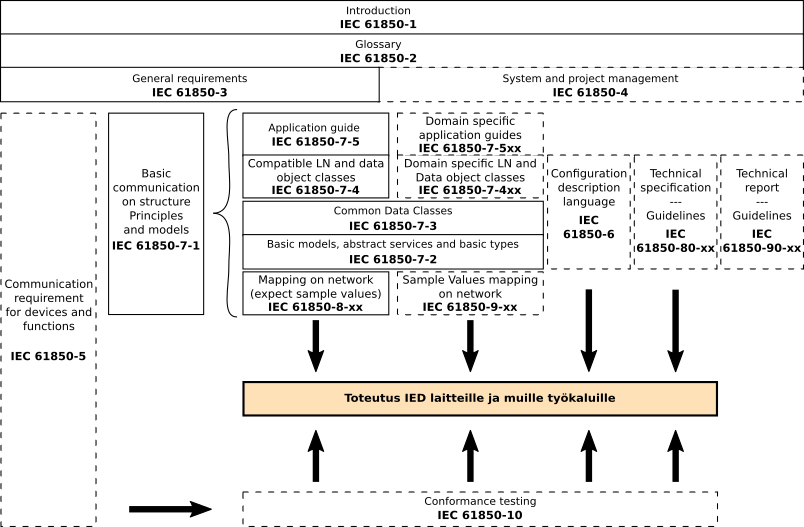
\includegraphics[width=1\textwidth]{pictures/iec61850-series-parts-and-relations.png}
	\caption{IEC 61850 -standardin osat ja niiden väliset relaatiot \cite[s.~14]{IEC61850-7-1} \cite[s.~22]{IEC61850-1}.}
	\label{fig:iec61850-osat-ja-relaatiot}
\end{figure}

Standardin ensimmäiset osat 1--5 kattavat yleistä kuvaa standardista ja sen vaatimuksista. Osiossa 6 käsitellään IED-laitteiden konfigurointiin käytetty XML (engl. Extensible Markup Language) -pohjainen kieli \cite[s.~7--8]{IEC61850-6}. Tämä osuus ei ole tämän työn kannalta tärkeä ja sitä ei sen tarkemmin käsitellä. Osat 7.1--7.4 käsittelevät standardin abstraktia mallia, niiden palveluita ja kuinka se rakentuu. Abstrahoidut palvelut standardissa lyhennetään ACSI (engl. Abstract Communication Service Interface), ja samaa lyhennettä käytetään tässä työssä \cite[s.~72]{IEC61850-7-1}. Osissa 8--9 ja niiden alakohdissa käsitellään abstraktimallien mallintamista erillisille protokollille, jolloin malleista tulee kyseisestä tekniikasta riippuvaisia. Abstrakteja malleja ja niiden mallintamista tekniikalle käsitellään teoriassa erikseen. Osa 10 käsittelee testausmenetelmiä, joilla voidaan varmistaa standardin määritysten noudattaminen. Tämä osuus ei myöskään ole tämän työn kannalta tärkeä, ja sitä ei teoriassa sen takia käsitellä. \cite[s.~15]{IEC61850-7-1}


\subsection{Abstraktimalli ja sen osat}
\begin{it}
	Kirjoita tähän aseman funktioiden, fyysisen laitteiden ja loogisten noodien suhteesta toisiinsa. Kuva myös piirrä ja mallia ja tietoa tähän ota \cite[s.~19]{IEC61850-1}. Tälle tarve jos teksti ei ole muuten tarpeeksi ymmärrettävä.

	Piirrä tähän itse esimerkkikuva kuinka standardi mallintaa fyysisen laitteen loogisiksi laitteiksi. Ota mallia standarin 7-1 kuvasta sivulla 17.
\end{it}

IEC 61850 -standardin lähtökohtana on pilkkoa koko sähköaseman toiminnalisuuden funktiot pieniksi yksilöiksi. Pilkotut yksilöt abstrahoidaan ja pidetään sopivan kokoisina, jotta ne voidaan konfiguroida esitettäväksi erillisellä IED-laiteella. Yksi aseman funktio voidaan hajauttaa monelle eri IED-laitteelle. Esimerkiksi linjan suojaukseen liittyvät komponentit, katkaisija (engl. circuit braker) ja ylivirtasuoja (engl. overcurrent protection) omilla IED-laitteillaan. Toimiakseen, laitteiden täytyy vaihtaa informaatiota keskenään \cite[s.~31]{IEC61850-7-1}. Näitä pilkottuja yksilöitä kutsutaan standardissa nimellä looginen noodi (engl. logical node ja lyhennetään LN). Loogiset noodit siis mallinetaan jostakin systeemin käsiteellisestä osasta. Loogisia noodeja käytetään rakentamaan looginen laite (engl. logic device, lyhennetään LD). Looginen laite on aseman ohjausyksikkö ja jokin fyysisen laitteen osa, joka toteuttaa loogisten noodien ohjauksen yhtäaikaa. Ylläolevasta esimerkistä looginen laite olisi aseman linjan suojaukseen liittyvät osat sisältä laite. Looginen laite siis vastaa aseman fyysistä laitetta, joka on kytketty aseman verkkoon ja sillä on IP-osoite. Yksi aseman fyysinen laite voi hoitaa monen loogisen laitteen funktionaalisuuden. Kuvassa \ref{fig:iec61850-data-modeling} on esitetty standardin mallin eri osien hierarkia ja kuinka ne rakentuvat \cite[s.~2]{Camachi2017} \cite[s.~24]{IEC61850-1}.

\begin{figure}
	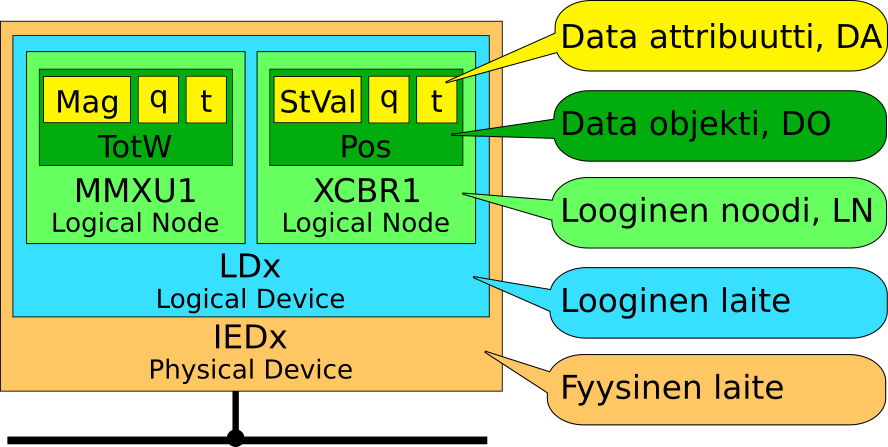
\includegraphics[width=1\textwidth]{pictures/iec61850-data-modeling.png}
	\caption{IEC 61850 -standardin abstraktimallin osat ja niiden hierarkia.}
	\label{fig:iec61850-data-modeling}
\end{figure}

Standardin määrittämissä osien hierarkiassa looginen laite on ylin yksilö, joka sisältää loogisia noodeja. Kuvassa \ref{fig:iec61850-data-modeling} IEDx ja LDx vastaavasti. Looginen noodi sisältää data objekteja (engl. data object, lyhennetään DO). Kuvassa \ref{fig:iec61850-data-modeling} loogiset noodit XCBR1 ja MMXU1. Ja data objektit Pos ja TotW. Data objekti sisältää data attribuutteja (engl. data attribute, lyhennetään DA). Kuvassa \ref{fig:iec61850-data-modeling} StVal, Mag, q ja t. Data objekti on tapa koostaa yhteen samaan asiaan liittyvät data attribuutit. Data attribuutit ovat laitteen konfiguroitavia ja luettavia datapisteitä. Data attribuutit kuvaavat esimerkiksi fyysisen laitteen tilaa ja mittausarvoja. Esimerkiksi mitattua jännitettä tai katkaisimen tilaa (kiinni tai auki). Standardin määrittämät data- objektit ja attribuutit voidaan lajitella 5 eri ryhmään:
\begin{itemize}
	\item yleinen loogisen noodin informaatio,
	\item tila informaatio,
	\item asetukset, 
	\item mitatut arvot ja
	\item ohjaus \cite[s.~25]{IEC61850-1}.
\end{itemize}

Tässä vaiheessa on hyvä mainita, että standardi pyrkii esittämään aseman funktioiden toiminnallisuutta hierarkialla ja oliopohjaisesti. Oliopohjaisesti siten, että standardi määrittää valmiita luokkia erilaisille loogisille noodeille. Esimerkiksi katkaisijalle on määritelty luokka nimeltä XCBR (circuit braker) \cite[s.~105--106]{IEC61850-7-4}. Ja mittaukselle MMXU (measurement) \cite[s.~57--58]{IEC61850-7-4}. Kun aseman toiminnallisuutta esitetään konfiguraatiossa ja IED-laitteella, luokia instanssioidaan tarpeen mukaan. Esimerkiksi kuvassa \ref{fig:iec61850-data-modeling} aikaisemmin mainitut loogisen noodin luokat on instansioitu nimellä XCBR1 ja MMXU1.

Standardi määrittää todella paljon erilaisia valmiita luokkia erilaisille loogisille noodeille valmiina käytettäväksi. Standardi myös määrittää laajenoksien mahdollisuudet luokkia käyttäen. Kaikki määritetyt luokat loogisille noodeille voi löytää standardin osasta 7-4.


\subsection{Loogisen noodin luokkien ja attribuuttien rakentuminen}
\begin{it}
	Ennen kirjoittamista lue 7-2 osuus ja selvitä meta-luokat standardista ja mitä ne pohjalla määrittävät ennen CDC-luokkia. Sen jälkeen kirjoita tähän kuinka standardin loogiset noodit rakentuvat. Kerro mitä common data classes sisältää ja kuinka ne määrittää data monessa paikassa käytetyt data attribuutit. Tämän jälkeen kuinka loogisen noodin luokat rakennetaan käyttämällä CDC määrityksiä \cite[s.~26]{IEC61850-1}. Ota tähän myös kuvia taulukosta ja rakenna esimerkkinä yksi looginen noodi niitä käyttäen. Tätä samaa mallia voi myöhemmin käyttää määrittämään kuinka referensssipolut luokkien nimillä rakentuu.
	Mallia loogisen noodin rakentamiseen voi myös ottaa \cite[s.~27]{IEC61850-7-1}.

	Kuvat:
	Kuva tai taulukko common data classin kentistä, logical noden kentistä mitä käytetään.
	Kuva lopullisen loogisen noodin luokan attribuuteista.
\end{it}

IEC 61850 -standardissa määritettyjen luokkien rakennetta on lähestytty oliopohjaisesti. Kaikki luokat määritellään standardissa taulukoilla, joissa on standardoitu kentän nimi, tyyppi, selitys ja onko kenttä optionaalinen Standardissa osassa 7-4 on lista kaikista sen määrittämistä loogisen noodin luokista eri tarkoituksiin. 

Loogisen noodin luokan kentät, kuten Pos, rakentuvat standardin yleisistä luokista (engl. Common Data Class, lyhennetään CDC). CDC-luokat ovat luokkia jotka sisältävät data attribuutteja, ja ovat yhteisiä monelle eri määritykselle. CDC-luokkien määritykset löytyy standardin osasta 7-3.

Kuvassa \ref{fig:xcbr-class} on esitetty standardin XCBR-luokan määritys taulukkomuodossa. Taulukko määrittää luokan kentät ja niiden nimet. Taulukon viimeinen sarake M/O/C, kertoo onko kenttä pakollinen (Mandatory, M), optionaalinen (Optional, O), vai konditionaalinen (Conditional, C). Taulun

\begin{figure}
	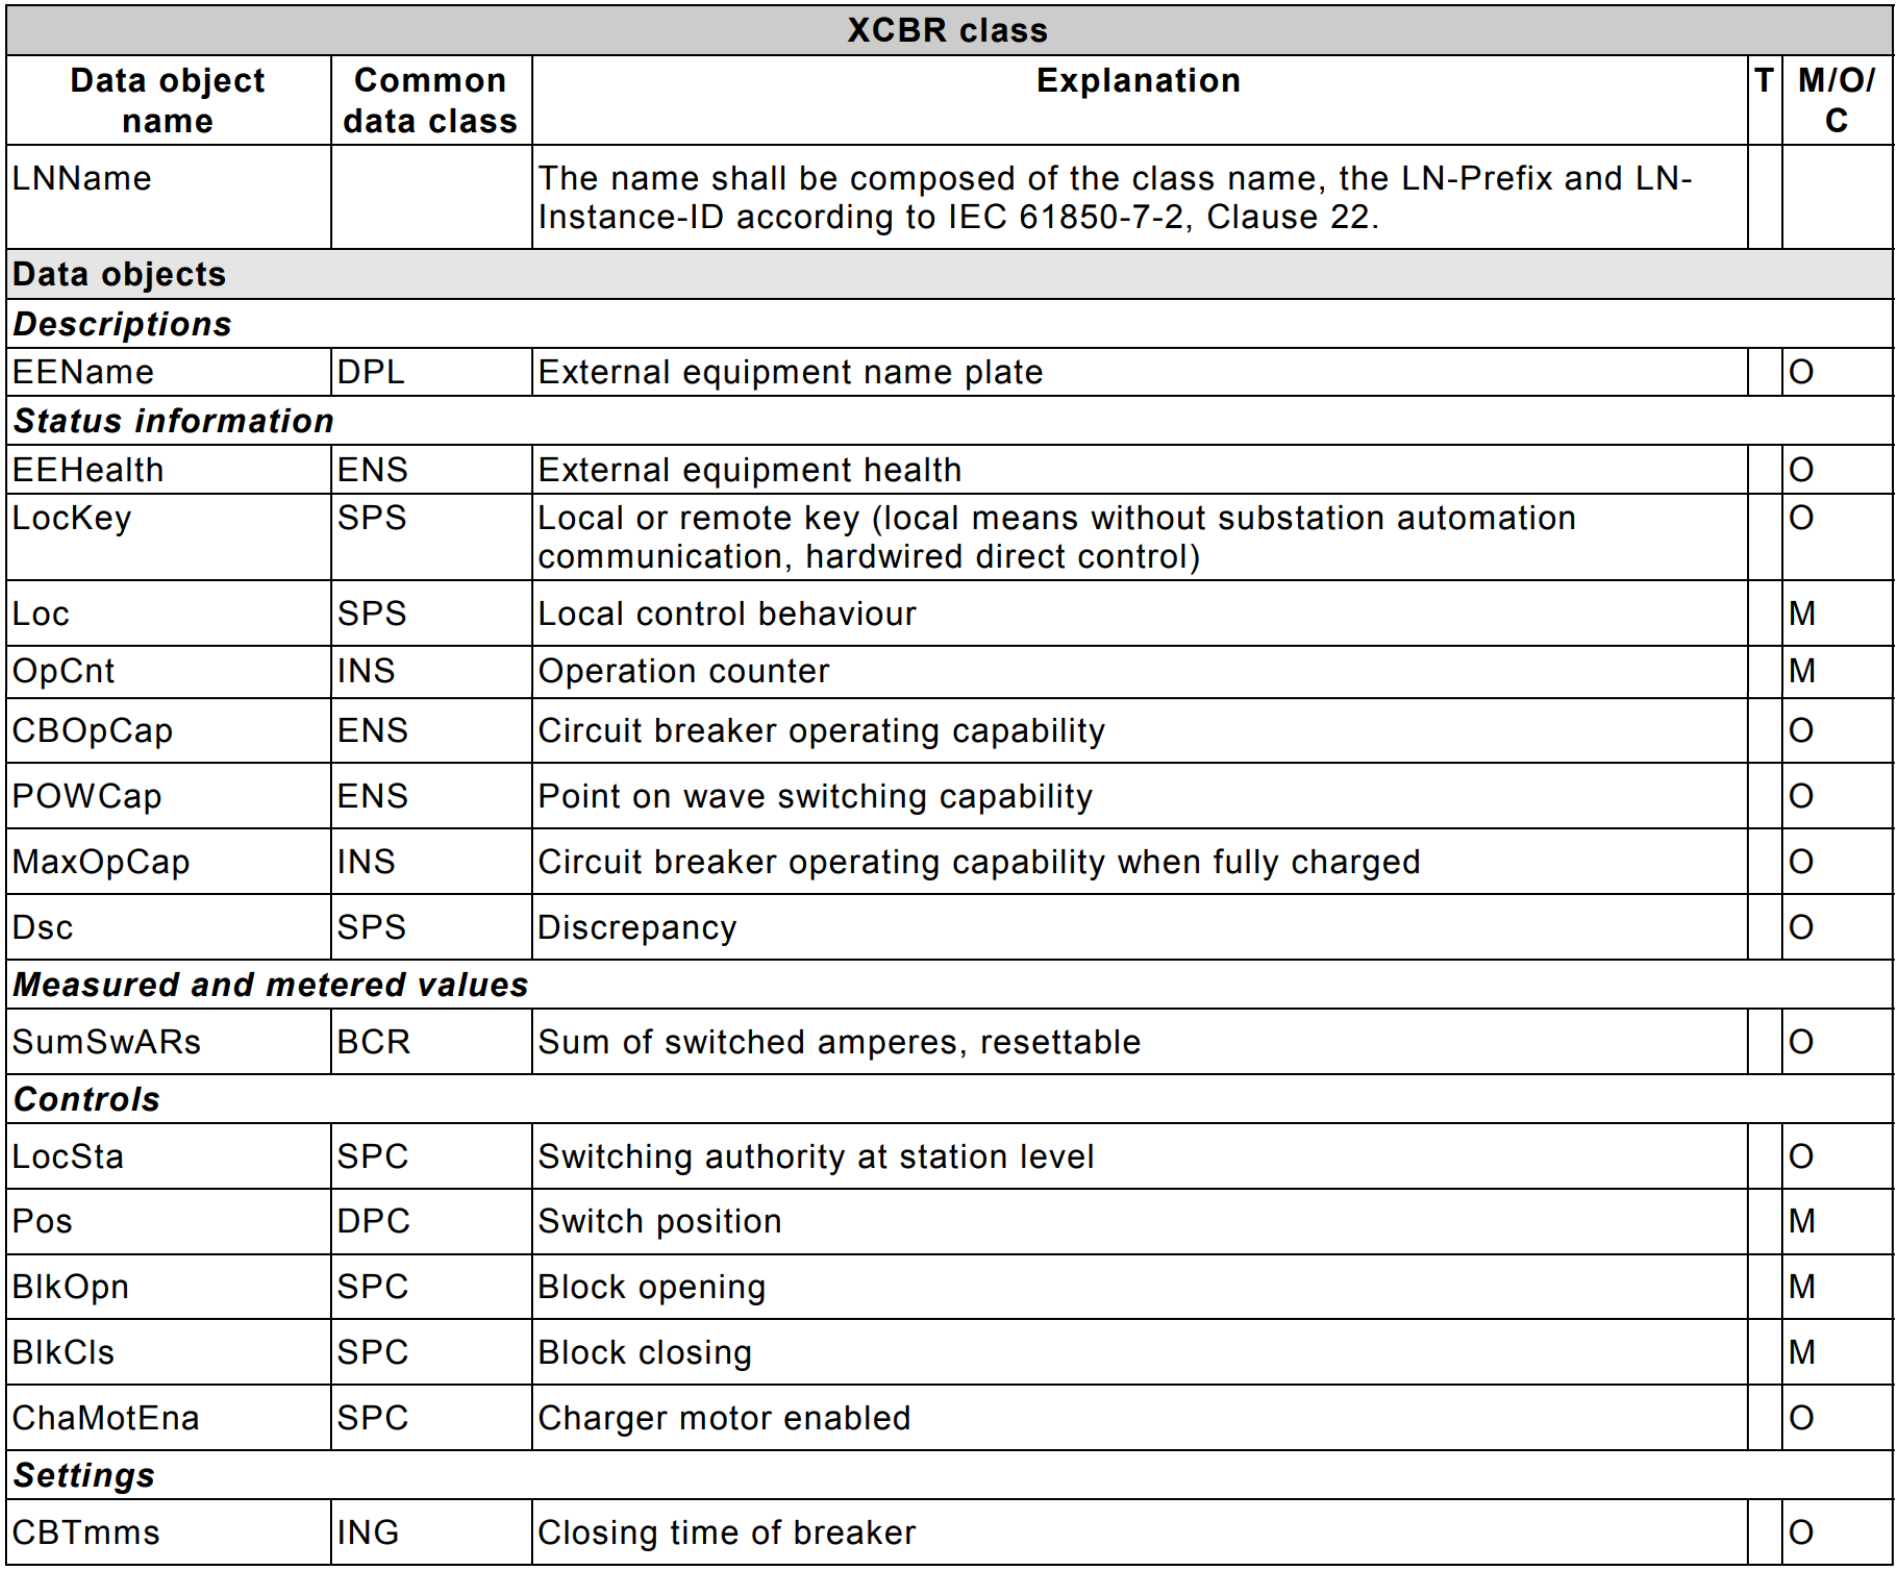
\includegraphics[width=1\textwidth]{pictures/xcbr-class.png}
	\caption{IEC 61850 -standardin katkaisijaluokan XCBR -määritys \cite[s.~106]{IEC61850-7-4}.}
	\label{fig:xcbr-class}
\end{figure}


\subsection{Attribuuttien viittaus hierarkiassa}
IEC 61850 -standardi määrittää tarkasti kuinka hierarkian eri kohtia viitataan IED-laitteessa. Viitteitä käytetään kun IED-laitteelle tehdään standardin osan 7-2 ACSI-määritysten mukaisia palvelukutsuja. Esimerkiksi jonkin attribuutin arvon asettaminen (SetDataValues) tai lukeminen (GetDataValues). Viitteen avulla IED-laite tietää, mihin loogisen noodin instanssiin ja sen data attribuuttiin palvelypyyntö kohdennetaan. Kuvassa \ref{fig:iec61850-data-reference} on esitetty kuinka standardi määrittää viitteen muodostumisen loogisesta laitteesta data attribuuttiin asti \cite[s.~93]{IEC61850-7-1}.

\begin{figure}
	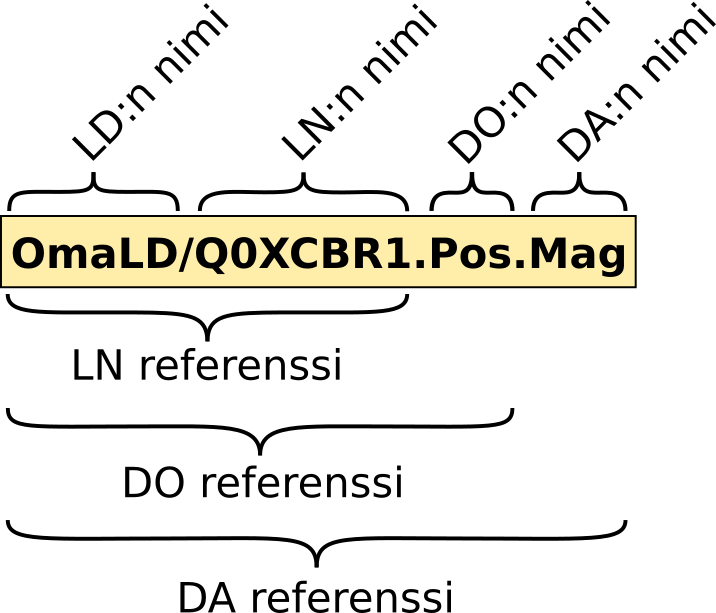
\includegraphics[width=0.5\textwidth]{pictures/iec61850-data-reference.png}
	\caption{IEC 61850 -standardin määrittämä viitteen rakenne.}
	\label{fig:iec61850-data-reference}
\end{figure}

Viite muodostuu suoraan laitteessa olevien luokkien instanssien nimien ja hierarkian mukaan. Loogisen laitteen (LD) ja loogisen noodin (LN) erottimena käytetään kauttaviivaa, ja muiden osien erottimena käytetään pistettä. Loogisella laitteella voi olla käyttäjän oma määrittämä nimi, mutta kuitenkin alle 65 merkkiä. Loogisen laitteen nimeen standardi ei puutu. Loogisen noodin instanssin nimi koostuu alku-, keski- ja loppuosasta. Alkuosan käyttäjä voi itse päättää, kuvassa \ref{fig:iec61850-data-reference} "\emph{Q0}". Voi sisältää numeroita ja kirjaimia, mutta täytyy alkaa kirjaimella. Keskiosan täytyy olla loogisen luokan nimi, josta instanssi on tehty. Tässä tapauksessa jo aikaisemmin mainittu katkaisijan luokka, XCBR. Tämä osuus on aina 4 kirjainta pitkä ja on aina isoilla kirjaimilla. Loppuosa on instanssin numeerinen arvo, joka ei sisällä kirjaimia. Loppuosan käyttäjä voi itse päättää, jonka ei tarvitse välttämättä olla juokseva numero. Alku- ja loppuosaan muotoon standardi ei anna määrityksiä. Alku- ja loppuosan yhteenlaskettu merkkien pituus täytyy olla alle 13 merkkiä. Data objektien (DO) ja attribuuttien (DA) niminä käytetään standardin määrittämiä nimiä, jotka määritetään niitä vastaavissa luokissa osissa 7-3 ja 7-4. Riippuen viittauksesta, näistä muodostuu loogisen noodin referenssi, data objektin referenssi ja data attribuutin referenssi. \cite[s.~181--182]{IEC61850-7-2} \cite[s.~93--95]{IEC61850-7-1}

Standardissa määritetään kaksi näkyvyysaluetta (engl. scope) viittaukselle, jotka ovat palvelin- ja looginen laite -näkyvyysalueet. Serverinäkyvyysalueelle viitataan ottamalla viittauksesta pois loogisen laitteen nimi. Eli kuvassa \ref{fig:iec61850-data-reference} viittaus tulisi muotoon "\emph{/Q0XCBR1.Pos.Mag}". Edellemainittua viittausta käytetään silloin, kun loogisen noodin instanssi sijaitsee loogisen laitteen ulkopuolella, mutta kuitenkin palvelimelta. Looginen laite -näkyvyysalueessa viittaus sisältää loogisen laitteen nimen ennen kauttaviivaa, toisin kuin palvelin-näkyvyysalueessa. Esimerkiksi kuvassa \ref{fig:iec61850-data-reference} oleva viittaus "\emph{OmaLD/Q0XCBR1.Pos.Mag}". Loogisen laitteen -näkyvyysaluetta käytetään silloin kun loogisen noodin instanssi sijaitsee loogisen laitteen sisällä sen hierarkiassa. Tässä työssä jatkossa käytetään pelkästään loogisen laitteen -näkyvyysaluetta. \cite[s.~183]{IEC61850-7-2}

Standardi määrittä maksimipituuksia viittauksille. Seuraavaksi kerrotut pituusmääritykset ovat voimassa kummallekin edelle mainitulle näkyvyysalueen viittaukselle. Ennen kauttaviivaa saa olla maksimissaan 64 merkkiä. Tämän jälkeen kauttaviiva, josta seuraa uudelleen maksimissaan 64 merkkiä. Eli koko viittauksen maksimipituus saa olla enintään 129 merkkiä, kauttaviiva mukaan lukien. \cite[s.~183]{IEC61850-7-2}


\subsection{Attribuuttien funktionaalinen rajoitus ja niistä muodostetut datajoukot}
\begin{it}
	Kirjoita tähän kuinka standardin mukaisia data settejä muodostetaan ja mitä ne ovat. Kirjoita tähän myös FCD ja FCDA lyhenteistä ja mitä ne tarkoittavat. Anna esimerkki kuinka data setit muodostuu vaikka kuvalla. Näitä tietoja tarvitaan kun käsitellään raportointilohkoja ja niiden tarkailevia data attribuutteja.
	
	Kirjoita tähän myös funktionaalisista rajoitteista, mitä standardi määrittää data attribuuteille. Ja kuinka näitä käytetään FCD ja FCDA ryhmien muodostamiseen. Funktionaalisesta rajoitteesta ja FCD ja FCDA asioista on tietoa \cite[s.~54--55]{IEC61850-7-2}.
\end{it}

Standardin yleiset luokat (CDC) määrittävät käytettävät data attribuutit. Luokat määrittää myös jokaiselle data attribuutille aikaisemmin mainittun funktionaalinen rajoitteen (engl. \emph{functional constraint}, lyhennetään \textbf{FC}). Funktionaalinen rajoite kuvaa attribuutin käyttötarkoitusta ja sitä mitä palveluita attribuuttiin voidaan käyttää. Funktionaalinen rajoite voidaan ymmärtää niin sanottuna suodattimena data objektin data attribuuteille. Esimerkiksi kaikki attribuutit, jotka liittyvät laitteen tilaan (engl. status), niillä on funktionaalinen rajoite ST (standardissa engl. status information). Standardi määrittää paljon erilaisia funktionaalisia rajoitteita, jotka ovat kaikki kahden ison kirjaimen yhdistelmiä. Taulukossa \ref{tab:iec61850-functional-constraints} on esitetty joitain tärkeimpiä funktionaalisia rajoitteita. Funktionaalinen rajoite myös määrittä onko attribuutti kirjoitettava tai luettava.

\begin{table}[ht!]
	\caption{Osa IEC 61850 -standardin määrittämistä funktionaalisista rajoitteitteista (FC) \cite[s.~54]{IEC61850-7-2}.}
	\label{tab:iec61850-functional-constraints}
	\begin{tabular}{l | l | l | l}
		\hline
		\textbf{Lyhenne} & \textbf{Selite} & \textbf{Luettava} & \textbf{Kirjoitettava} \\
		\hline \hline
		ST & Laitteen tilatieto (status) & Kyllä & Ei \\
		MX & Mittaustieto (measurands) & Kyllä & Ei \\
		CF & Laitteen asetusarvo (configuration) & Kyllä & Kyllä \\
		DC & Selitystieto (description) & Kyllä & Kyllä \\
		\hline
	\end{tabular}
\end{table}

Funktionaalisia rajoitteita käytetään, kun IED-laitteeseen tehdään ACSI-palveluiden mukaisia kutsuja. Esimerkiksi jos halutaan lukea kuvassa \ref{fig:iec61850-data-reference} OmaLD/Q0XCBR1.Pos polussa olevan data objektin kaikki tilan arvot yhdellä kutsulla, käytettäisiin ST funktionaalista rajoitetta taulukosta \ref{tab:iec61850-functional-constraints}. Kutsu jättää lukematta kaikki muut data objektin attribuutit.

Funktionaalista rajoitetta voidaan käyttää suodattamaan data attribuutteja data objektista ja niiden ali data objekteista. Toisin sanoen hierarkiassa referenssipisteestä alaspäin oleviin kentiin. Standardi määrittä lyhtenteen FCD (engl. Functional Constrained Data), jota käytetään silloin kun hierarkian ensimmäistä data objektia suodatetaan funktionaalisella rajoitteella. Aikaisemmin mainittu OmaLD/Q0XCBR1.Pos funktionaalisella rajoitteella ST, on FCD-suodatus. Tässä Pos on ensimmäinen data objekti Q0XCBR1 loogisen noodin jälkeen.

\begin{it}
	Kirjoita yllä olevaan kappaleeseen vielä FCDA määrityksestä ja sitten tämän jälkeen kuinka FCD ja FCDA määrityksiä käytetään datajoukkojen rakentamiseen IED-laitteeseen. Piirrä tähän myös kuva, josta tulee esille FCD:n ja FCDA:n erot ja kuinka se suodattaa.
\end{it}	

\subsection{Abstrakti kommunikointi ja ACSI}
\begin{it}
	Voisiko tähän kirjoittaa miten mappaus johonkin tekniikkaan tapahtuu ja kuinka kommunikaatio sitten tapahtuu oikeasti. Samalla selittää ACSI-mallista jotain. Hyvä kuva standardissa löytyy tästä löytyy \cite[s.~76]{IEC61850-7-1}. Voisiko tämän heittää johonkin omana otsikkonaan?
	
	Voisiko tähän myös laittaa kuva kuinka osat on pilkottu eri IED-laitteille ja niiden välinen kommunikoninti. Mallia \cite[s.~31]{IEC61850-7-1}.
\end{it}


\subsection{Viestien tilaus ja tilauksen konfigurointi}
\begin{it}
	Kirjoita tähän IEC 61850 -standardin määrittästä abstraktista raportointimallista. Tätä raportointi mekanismia tullaan käyttämään raporttien tilauksessa ja sen konfigurointi täytyy ymmärtää toteuttettavan ohjelmiston kannalta. Käy läpi mitä asiakasohjelman täytyy tehdä ja mikä on tapahtumien järjestys jotta raportteja voidaan edes tilata.
	Hyvä kuva ja selitys missä järjestyksessä asiat tapahtuu asiakkaan ja palvelimen välillä. Ja yleistä tietoa raportoinnista löytyy \cite[s.~40--44]{IEC61850-7-1}.
	
	Kirjoita data attribuuttien liipaisimiin enemmän laadun muutoksesta mitä tarkoittaa ja viite sinne.
\end{it}

IEC 61850 -standardi määrittää erilaisia liipaisimia data attribuuteille, joita voidaan käyttää liipaisemaan jokin tapahtuma IED-laitteessa. Standardi määrittää seuraavia liipaisimia data attribuuteille:
\begin{itemize}
	\item datan muutos (engl. data change, standardissa lyhenne \emph{dchg}),
	\item laadun muutos (engl. quality change, standardissa lyhenne \emph{qchg}), ja
	\item datan päivitys (engl. data update, standardissa lyhenne \emph{dupd}).
\end{itemize}
Edellä mainituissa ero datan muutoksen ja päivityksen välillä on se, että datan päivitys liipaisee tapahtuman, vaikka attribuutin uusi arvo olisi sama. Datan muutos ei liipaise tapahtumaa, jos uusi arvo on sama kuin edellinen arvo. Laadun muutos tarkoittaa, että data attribuuttiin liitetty laatuarvo muuttuu. Laatuarvo kertoo, voiko attribuutin arvoon luottaa. \cite[s.~90]{IEC61850-7-1}

Standardi määrittää kaksi mahdollisesti liipaistavaa tapahtumaa IED-laitteessa, jotka ovat raportointi ja lokitus. Lokitus on IED-laiteessa tapahtuvien tapahtumien lokitusta myöhempää käyttöä ja tarkastelua varten. Esimerkiksi attribuutin arvon muutos. Raportointi on tapahtuma, jossa generoidaan viesti tapahtuman liipaisseista attribuuteista. Tämä viesti lähetetään niitä tilaaville asiakkaille. Jos tilaavaa asiakasta ei ole, viestiä ei generoida. Standardi käyttää sanaa "raportti" (engl. ja standardissa report) näiden viestien kuvaamiseen. Kuitenkin tässä työssä on käytetty sanaa "viesti" tästä eteenpäin "raportin" sijaan. Tämä sen takia, koska suomenkielessä raportti-sana voi tarkoittaa lukijalle muuta merkitystä, kuin verkon yli asiakkaan ja palvelimen välistä viestiä. Tässä työssä keskitytään edelle mainittuihin viesteihin, ei lokitukseen. Ja lopullinen ohjelmisto nimenomaan käsitteli näitä viestejä.

Standardi määrittelee kaksi luokkaa viestien tilaamisen ja konfigurointiin. Luokat ovat puskuroitu viestintälohko (engl. \emph{Buffered Report Control Block}, lyhennetään \textbf{BRCB}) ja ei puskuroitu lohko (engl. \emph{Unbuffered Report Control Block}, lyhennetään \textbf{URCB}). Tekstissä kumpaakin luokkaan viitatessa käytetään lyhennettä \textbf{RCB}. Ainoa ero luokkien välillä on, että BRCB puskuroi viestejä jonkin aikaa yhteyden katkettua. Yhteyden palautuessa, se lähettää puskuroidut viestit järjestyksessä asiakkaalle. BRCB takaa viestien järjestyksen ja saatavuuden. URCB lähettää viestejä asiakkaalle ilman puskurointia. Yhteyden katketessa, viestit menetetään. IED-laitetta konfiguroitaessa, luokista tehdään instansseja asiakkaiden tarpeen mukaan. Standardi määrittää, että tilaavan asiakkaan on varattava yksi RCB-instanssi itselleen ja tänä aikana muut asiakkaat eivät voi kyseistä RCB:tä käyttää. Niinpä IED-laitteelle on määritettävä RCB-instansseja sen käyttötarkoitusten mukaan.

Jokainen RCB-instanssi kytketään johonkin muodostettuun datajoukkoon, jota se tarkkailee ja josta viestit generoidaan. Yhteen datajoukkoon voi olla kytkettynä monta RCB-instanssia. Jolloin yhden data attribuutin liipaistessa, jokainen siihen kytketty RCB generoi viestin asiakkaalle.

RCB-luokat sisältävät attribuutteja, joita asiakas konfiguroi ennen tilausta omien tarpeidensa mukaan. Tämän jälkeen asiakas varaa RCB:n kirjoittamalla konfiguroidut arvot ja asettamalla kentän RptEna arvoksi tosi (katso taulukko \ref{tab:iec61850-brcb-class-definition}). Tämän jälkeen RCB on varattu kyseiselle asiakkaalle ja IED-laite aloittaa datajoukon attribuuttien tarkkailun. Asiakas jää odottamaan viestien tuloa palvelimelta ilman erillistä kyselyä. Jos konfiguroitu liipaisin liipaisee tapahtuman, RCB lähettää viestin asiakkaalle. Kuvassa \ref{fig:iec61850-brcb-communication} on esitetty yllämainittu prosessi asiakkaan ja palvelimen välillä käyttäen puskuroitua BRCB-luokkaa. Kuvassa yhteyden katketessa, palvelin puskuroi viestejä. Yhteyden palautuessa samalta asiakkaalta, palvelin lähettää viestit oikeassa järjestyksessä asiakkaalle. Tilaus lopetetaan asiakkaan pyynnöstä tai yhteyden ollessa poikki tarpeeksi kauan.

\begin{figure}
	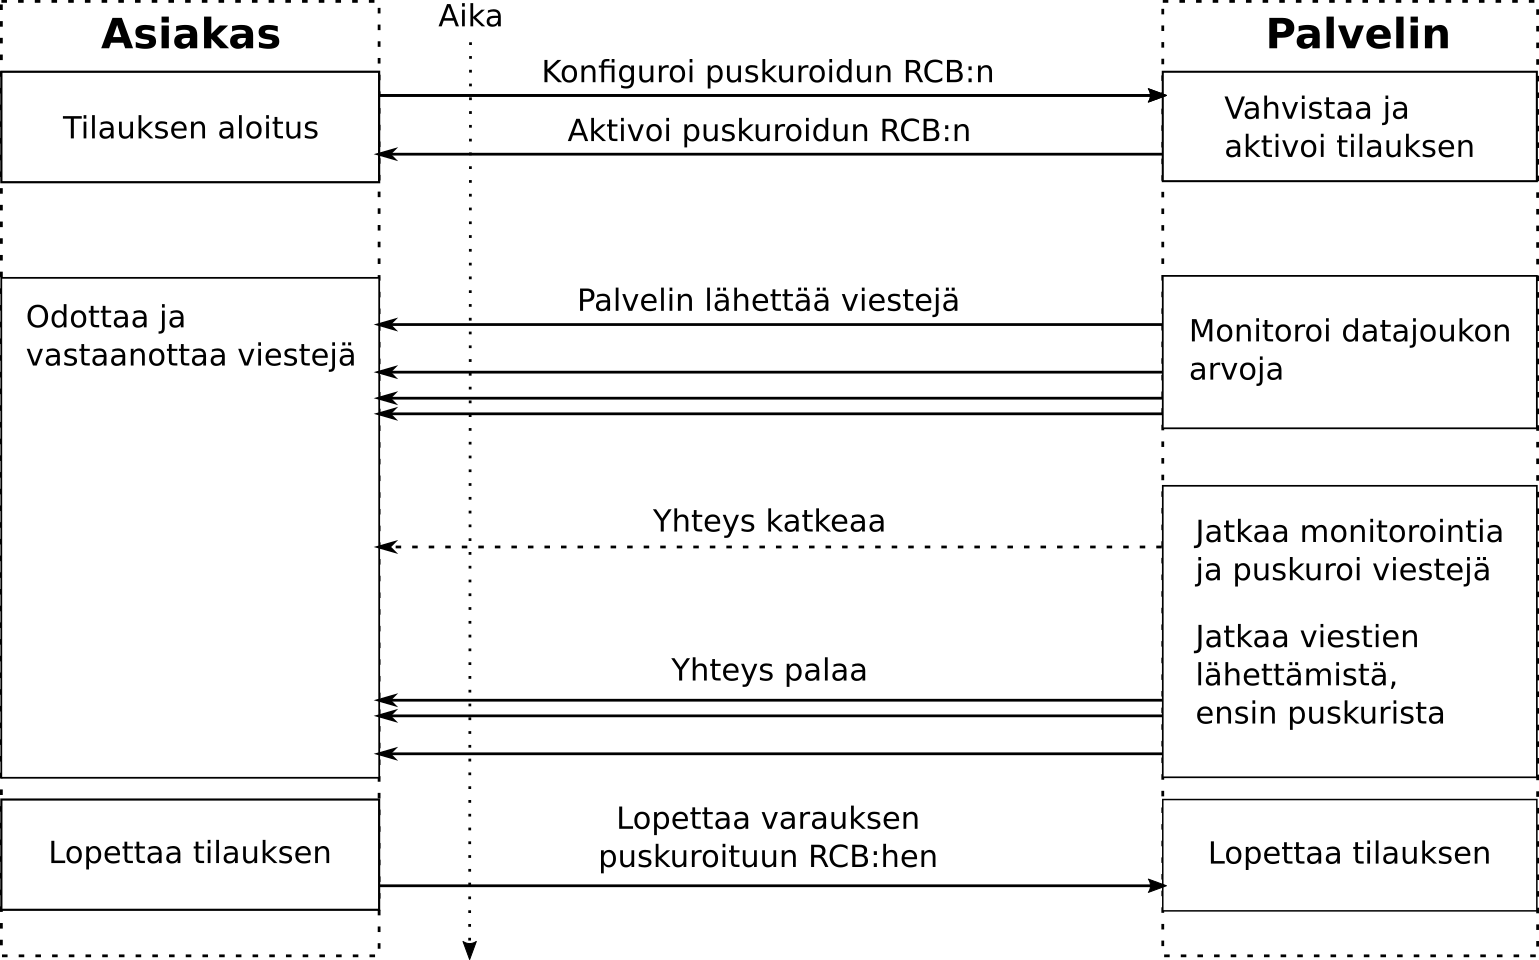
\includegraphics[width=1\textwidth]{pictures/iec61850-brcb-communication.png}
	\caption{Puskuroitu viestien tilausprosessi asiakkaan ja palvelimen välillä.}
	\label{fig:iec61850-brcb-communication}
\end{figure}


\subsection{Raportointi-luokan määritys ja toiminta}
\begin{it}
	Kirjoita tähän standardin määritämästä BRCB luokan rakenteesta ja mitä tietoa se sisältää.
	Mainitse että standardissa käytetään UTC-aikaa aikakentissä \cite[s.~50]{IEC61850-7-1}.
\end{it}

BRCB-luokalla on erilaisia attribuutteja, joita asiakas voi kirjoittaa ja lukea ennen tilauksen aloittamista. Taulukossa \ref{tab:iec61850-brcb-class-definition} on esitetty standardin määrittämän BRCB-luokan attribuutit, attribuutin nimi englanniksi ja sen selite. Taulukossa ei ole esitetty attribuuttien tyyppejä, koska ne voi lukija tarvittaessa tarkemmin lukea standardin omasta määrityksestä. Ja standardissa muutenkin kuvataan luokan eri attribuuttien toiminta paljon perusteellisemmin. Tässä työssä riittää että lukija ymmärtää luokan päätoiminnan hyvin. URCB-luokka on melkein samanalainen kuin taulukossa \ref{tab:iec61850-brcb-class-definition} määritetty BRCB-luokka. Tarkka määritys ja BRCB ja URCB luokkien erot löytyvät standardin osasta 7-2 \cite[s.~93--118]{IEC61850-7-2}.

\begin{table}[ht!]
	\caption{BRCB-luokan määritetyt attribuutit ja niiden selitteet \cite[s.~94--103]{IEC61850-7-2}.}
	\label{tab:iec61850-brcb-class-definition}
	\begin{tabular}{l | l | l}
		\hline
		\textbf{Attribuutti} & \textbf{Englanniksi} & \textbf{Selite} \\
		\hline \hline
		BRCBName & BRCB name & Objektin nimi \\
		BRCBRef & BRCB reference & Objektin referenssi \\
		RptID & Report identifier & \parbox[t]{7.5cm}{RCB-instanssin yksilöivä id lähetettyihin viesteihin, asiakas voi asettaa} \\
		RptEna & Report enable & Varaa RCB:n ja aloittaa viestien lähetyksen \\
		DatSet & Data set reference & Tarkailtavan datajoukon referenssi \\
		ConfRev & Configuration revision & \parbox[t]{7.5cm}{Juokseva configuraation numerointi, muutos kasvattaa numerointia} \\
		OptFlds & Optional fields & Mitä optionaalisia kenttiä viestiin lisätään \\
		BufTm & Buffer time & \parbox[t]{7.5cm}{Puskurointiaika, ennen viestin lähetystä. Tänä aikana tapahtuvat liipaisut yhdistetään samaan viestiin} \\
		SqNum & Sequence number & Juokseva lähetetyn viestin numerointi \\
		TrgOps & Trigger options & Millä liipaisimilla viesti lähetetään \\
		IntgPd & Integrity period & \parbox[t]{7.5cm}{Periodisen viestien väli millisekunteina, arvolla 0 ei käytössä} \\
		GI & General-interrogation & \parbox[t]{7.5cm}{Käynnistää yleiskyselyn, joka sisältää kaikki datajoukon attribuutit seuraavaan viestiin} \\
		PurgeBuf & Purge buffer & Puhdistaa lähettämättömät viestit puskurista \\
		EntryID & Entry identifier & \parbox[t]{7.5cm}{Puskurissa olevan viimeisimmän viestin id. Arvo 0 tarkoittaa tyhjää puskuria} \\
		TimeOfEntry & Time of entry & \parbox[t]{7.5cm}{Puskurissa olevan viimeisimmän viestin aikaleima} \\
		ResvTms & Reservation time & \parbox[t]{7.5cm}{Varausaika millisekunteina, arvo -1 tarkoittaa konfiguraation aikaista varausta ja 0 että ei varausta} \\
		Owner & Owner & \parbox[t]{7.5cm}{Yksilöi varaavan asiakkaan, yleensä IP-osoite tai IED-laitteen nimi. Arvo 0 että RCB on vapaa tai ei omistajaa} \\
		\hline
	\end{tabular}
\end{table}

RCB-luokan TrgOps-attribuutti on binääritietue, jossa yksittäinen bitti ilmaisee mikä liipaisin voi aiheuttaa viestin lähettämisen. Asiakas voi päättää mitä liipaisimia haluaa käyttää. TrgOps sisältää seuraavat liipaisimet:
\begin{itemize}
	\item datan muutos (engl. data change, standardissa lyhenne \emph{dchg}),
	\item laadun muutos (engl. quality change, standardissa lyhenne \emph{qchg}), ja
	\item datan päivitys (engl. data update, standardissa lyhenne \emph{dupd}),
	\item yleinen kysely (enlg. \emph{general-interrogation}, standardissa lyhenne GI), ja 
	\item jatkuva viestintä väliajoin (engl. \emph{intergrity}).
\end{itemize}

Kolme ensimmäistä dchg, qchg ja dupd ovat aikaisemmin määrittettyjen data attribuuttien liipaisimia. Asiakas voi tilata viestejä esimerkiksi vain data muutoksista ja ei muista. RCB-luokka määrittää data attribuuttien liipaisimien lisäksi vielä kaksi liipaisinta lisää, yleinen kysely ja jatkuva viestintä väliajoin. Yleinen kysely on viesti, johon RCB sisällyttää kaikki datajoukon attribuutit. Ja jonka asiakas voi liipaista asettamalla luokan attribuutin GI arvoksi tosi ja TrgOps attribuutissa liipaisin on päällä. Tällöin RCB käynnistää viestin generoinnin ja lähettää sen asiakkaalle. Jos liipaisin ei ole päällä TrgOps attribuutissa, ja GI arvoksi asetetaan tosi. RCB ei generoi viestiä. Viestin lähetyksen jälkeen RCB itse asettaa GI:n arvoksi epätosi. Jatkuva viestintä on viestin lähettäminen asiakkaalle tietyn väliajoin, johon sisältyy kaikki datajoukon attribuutit, kuten yleisessä kyselyssä. Toiminnon saa päälle kun asiakas asettaa RCB-luokassa attribuutit IntgPd arvoksi muu kuin 0, ja TrgOps attribuutin arvossa kyseinen liipaisin on päällä. Attribuutti IntgPd kertoo minkä väliajoin viesti generoidaan ja lähetetään asiakkaalle. Jos IntgPd arvo on muu kuin 0 ja TrgOps atribuutissa liipaisin ei ole päällä, ei viestiä generoida ja lähetetä asiakkaalle väliajoin.

Viestien tilaus aloitetaan kun asiakas kirjoittaa RptEna-attribuutin arvoksi tosi. Tilauksen aikana kirjoitus joihinkin attribuutteihin muuttuu, verrattuna ennen tilausta. Esimerkiksi yleisen kyselyn tekeminen on mahdollista tilauksen aikana kirjoittamalla GI:n arvoksi tosi. Tilauksen aikana kirjoittamalla TrgOps-attribuutin aiheuttaa puskurin tyhjentämisen. Ja Attribuutin OptFlds kirjoitus aiheuttaa epäonnistuneen vastauksen palvelimelta.

RCB-luokan attribuuttin OptFlds avulla asiakas voi asettaa mitä vaihtoehtoisia kenttiä viestiin sisällytetään. Attribuutin OptFlds on binääritietue, niin kuin ja TrgOps ja taulukossa \ref{tab:iec61850-optional-fields-definition} on esitetty sen asetettavat arvot \cite[s.~98]{IEC61850-7-2}.

\begin{table}[ht!]
	\caption{RCB-luokan OptFlds attribuutin arvot ja niiden selitteet,}
	\label{tab:iec61850-optional-fields-definition}
	\begin{tabular}{l | l}
		\hline
		\textbf{Arvo} & \textbf{Selite} \\
		\hline \hline
		sequence-number & Jos tosi, sisällytä RCB-luokan attribuutti SqNum viestiin \\
		report-time-stamp & Jos tosi, sisällytä RCB-luokan attribuutti TimeOfEntry viestiin \\
		reason-for-inclusion & Jos tosi, sisällytä syy miksi arvo(t) sisällytettiin viestiin \\
		data-set-name & Jos tosi, sisällytä RCB-luokan attribuutti DatSet viestiin \\
		data-reference & \parbox[t]{10cm}{Jos tosi, sisällytä datajoukon liipaisseen kohdan rakentamiseen käytetty FCD- tai FCDA-referenssi viestiin} \\
		buffer-overflow & \parbox[t]{10cm}{Jos tosi, sisällytä viestiin tieto onko puskuri vuotanut yli kentällä BufOvfl (engl. buffer overflow)} \\
		entryID & Jos tosi, sisällytä RCB-luokan attribuutti EntryID viestiin \\
		conf-revision & Jos tosi, sisällytä RCB-luokan attribuutti ConfRev viestiin \\
		\hline
	\end{tabular}
\end{table}

Kuinka attribuutit vaikuttavat viestin rakenteeseen ja mitä syitä arvon tai arvojen sisältymiseen viestissä voi olla, käsitellään seuraavassa kohdassa.


\subsection{Viestin rakenne ja muoto}
\begin{it}
	Kirjoita tähän standardin määritämästä viestin rakenteesta ja mitä optionaaliset kentät siihen vaikuttavat. Lisäksi selitä ReasonForInclusion arvosta ja mitä vaihtoehtoja sille on \cite[s.~28--29]{IEC61850-7-2}.
\end{it}

\begin{figure}
	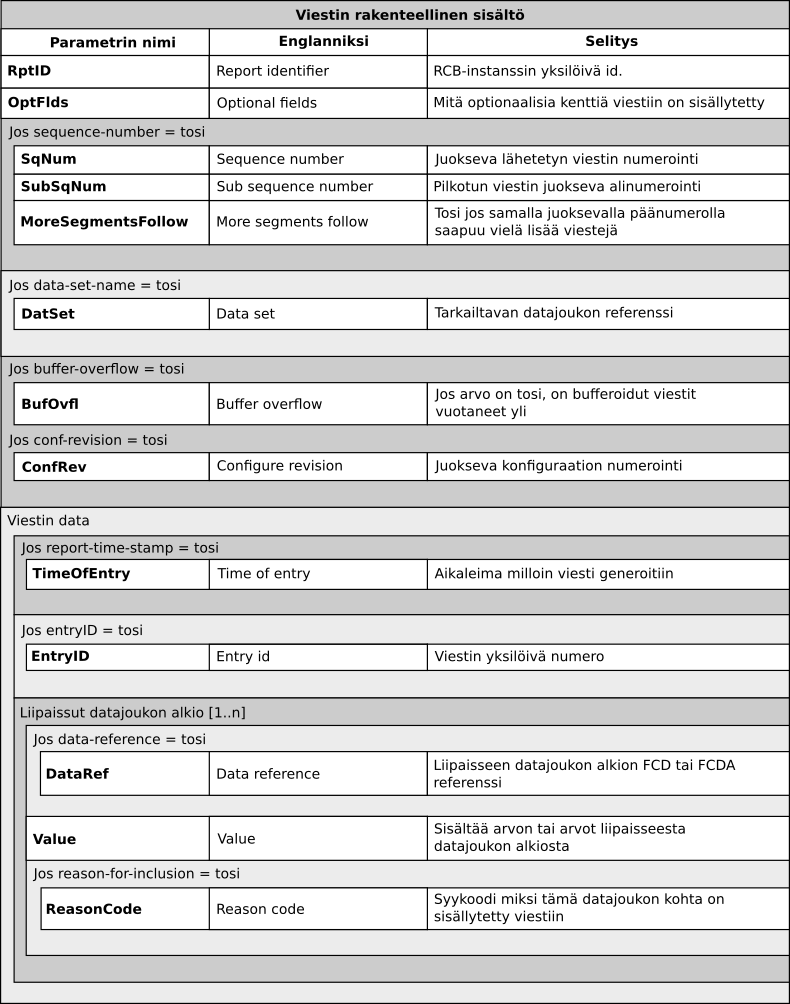
\includegraphics[width=1\textwidth]{pictures/iec61850-report-format.png}
	\caption{Standardin määrittämä lähetetyn viestin formaatti \cite[s.~104]{IEC61850-7-2}.}
	\label{fig:iec61850-report-format}
\end{figure}


\section{Abstraktimallin sovitus MMS-protokollaan}
\begin{it}
	Kirjoita kuinka ylempi ACSI sovitetaan MMS-protokollan palveluiksi ja tietotyypeiksi standardin IEC 61850-8-1 osuuden mukaan. Tähän myös miten raportointi toimii MMS-protokollan päällä.
\end{it}


\subsection{MMS-protokolla}
\begin{it}
	Selitä lyhyesti mikä on MMS-protokolla ja vähän sen tietotyypeistä. Tämän tarkoitus on pohjustaa tulevaa IEC 61850 abstraktien olioiden (ACSI) sovitusta tämän protokollan päälle.
\end{it}


\section{Advanced Message Queuing Protocol}
\begin{it}
	Kirjoita tähän AMQP määrittävästä standardista, mikä sen tarkoitus on ja mihin sitä voidaan käyttää.
\end{it}


\subsection{Viestien välitysmekanismit}
\begin{it}
	Mitä mekanismeja AMQP tarjoaa viestien välittämiseen osapuolille. Näitä on jono, reititys suoraan osapuolien välillä ja viestin julkaisu ja tilaaminen.
\end{it}


\subsection{Tilaus ja julkaisu -mallin osat}
\begin{it}
	Kirjoita tähän AMQP tarjoamista viestien julkaisu ja tilaus -mallin osista osapuolten kesken. Kerro mitä eri osat tekevät ja mikä niiden tehtävä viestien välittämisessä on. Englanniksi osia ovat esim. exchange, queue, publisher ja consumer.
\end{it}